\documentclass[twoside]{book}

% Packages required by doxygen
\usepackage{fixltx2e}
\usepackage{calc}
\usepackage{doxygen}
\usepackage[export]{adjustbox} % also loads graphicx
\usepackage{graphicx}
\usepackage[utf8]{inputenc}
\usepackage{makeidx}
\usepackage{multicol}
\usepackage{multirow}
\PassOptionsToPackage{warn}{textcomp}
\usepackage{textcomp}
\usepackage[nointegrals]{wasysym}
\usepackage[table]{xcolor}

% Font selection
\usepackage[T1]{fontenc}
\usepackage[scaled=.90]{helvet}
\usepackage{courier}
\usepackage{amssymb}
\usepackage{sectsty}
\renewcommand{\familydefault}{\sfdefault}
\allsectionsfont{%
  \fontseries{bc}\selectfont%
  \color{darkgray}%
}
\renewcommand{\DoxyLabelFont}{%
  \fontseries{bc}\selectfont%
  \color{darkgray}%
}
\newcommand{\+}{\discretionary{\mbox{\scriptsize$\hookleftarrow$}}{}{}}

% Page & text layout
\usepackage{geometry}
\geometry{%
  a4paper,%
  top=2.5cm,%
  bottom=2.5cm,%
  left=2.5cm,%
  right=2.5cm%
}
\tolerance=750
\hfuzz=15pt
\hbadness=750
\setlength{\emergencystretch}{15pt}
\setlength{\parindent}{0cm}
\setlength{\parskip}{3ex plus 2ex minus 2ex}
\makeatletter
\renewcommand{\paragraph}{%
  \@startsection{paragraph}{4}{0ex}{-1.0ex}{1.0ex}{%
    \normalfont\normalsize\bfseries\SS@parafont%
  }%
}
\renewcommand{\subparagraph}{%
  \@startsection{subparagraph}{5}{0ex}{-1.0ex}{1.0ex}{%
    \normalfont\normalsize\bfseries\SS@subparafont%
  }%
}
\makeatother

% Headers & footers
\usepackage{fancyhdr}
\pagestyle{fancyplain}
\fancyhead[LE]{\fancyplain{}{\bfseries\thepage}}
\fancyhead[CE]{\fancyplain{}{}}
\fancyhead[RE]{\fancyplain{}{\bfseries\leftmark}}
\fancyhead[LO]{\fancyplain{}{\bfseries\rightmark}}
\fancyhead[CO]{\fancyplain{}{}}
\fancyhead[RO]{\fancyplain{}{\bfseries\thepage}}
\fancyfoot[LE]{\fancyplain{}{}}
\fancyfoot[CE]{\fancyplain{}{}}
\fancyfoot[RE]{\fancyplain{}{\bfseries\scriptsize Generated by Doxygen }}
\fancyfoot[LO]{\fancyplain{}{\bfseries\scriptsize Generated by Doxygen }}
\fancyfoot[CO]{\fancyplain{}{}}
\fancyfoot[RO]{\fancyplain{}{}}
\renewcommand{\footrulewidth}{0.4pt}
\renewcommand{\chaptermark}[1]{%
  \markboth{#1}{}%
}
\renewcommand{\sectionmark}[1]{%
  \markright{\thesection\ #1}%
}

% Indices & bibliography
\usepackage{natbib}
\usepackage[titles]{tocloft}
\setcounter{tocdepth}{3}
\setcounter{secnumdepth}{5}
\makeindex

% Custom commands
\newcommand{\clearemptydoublepage}{%
  \newpage{\pagestyle{empty}\cleardoublepage}%
}

\usepackage{caption}
\captionsetup{labelsep=space,justification=centering,font={bf},singlelinecheck=off,skip=4pt,position=top}

%===== C O N T E N T S =====

\begin{document}

% Titlepage & ToC
\pagenumbering{alph}
\begin{titlepage}
\vspace*{7cm}
\begin{center}%
{\Large cpp\+\_\+arcade \\[1ex]\large 1.\+0 }\\
\vspace*{1cm}
{\large Generated by Doxygen 1.8.13}\\
\end{center}
\end{titlepage}
\clearemptydoublepage
\pagenumbering{roman}
\tableofcontents
\clearemptydoublepage
\pagenumbering{arabic}

%--- Begin generated contents ---
\chapter{arcade}
\label{md__r_e_a_d_m_e}
\section*{Libraries graphiques\+: }

S\+F\+ML 2.\+4.\+2; n\+Curses5; 
\chapter{Hierarchical Index}
\section{Class Hierarchy}
This inheritance list is sorted roughly, but not completely, alphabetically\+:\begin{DoxyCompactList}
\item \contentsline{section}{I\+Display\+Module}{\pageref{class_i_display_module}}{}
\begin{DoxyCompactList}
\item \contentsline{section}{lib\+\_\+\+N\+C\+U\+R\+S\+ES}{\pageref{classlib___n_c_u_r_s_e_s}}{}
\item \contentsline{section}{lib\+\_\+\+S\+F\+ML}{\pageref{classlib___s_f_m_l}}{}
\end{DoxyCompactList}
\item \contentsline{section}{I\+Load\+Game}{\pageref{class_i_load_game}}{}
\begin{DoxyCompactList}
\item \contentsline{section}{Snake}{\pageref{class_snake}}{}
\item \contentsline{section}{solarfox}{\pageref{classsolarfox}}{}
\end{DoxyCompactList}
\item \contentsline{section}{player}{\pageref{classplayer}}{}
\item \contentsline{section}{s\+\_\+core}{\pageref{structs__core}}{}
\item \contentsline{section}{s\+\_\+draw\+\_\+data}{\pageref{structs__draw__data}}{}
\item \contentsline{section}{s\+\_\+stock}{\pageref{structs__stock}}{}
\item \contentsline{section}{lib\+\_\+\+S\+F\+ML\+:\+:s\+\_\+textu}{\pageref{structlib___s_f_m_l_1_1s__textu}}{}
\end{DoxyCompactList}

\chapter{Class Index}
\section{Class List}
Here are the classes, structs, unions and interfaces with brief descriptions\+:\begin{DoxyCompactList}
\item\contentsline{section}{\textbf{ I\+Display\+Module} }{\pageref{class_i_display_module}}{}
\item\contentsline{section}{\textbf{ I\+Load\+Game} }{\pageref{class_i_load_game}}{}
\item\contentsline{section}{\textbf{ lib\+\_\+\+N\+C\+U\+R\+S\+ES} }{\pageref{classlib___n_c_u_r_s_e_s}}{}
\item\contentsline{section}{\textbf{ lib\+\_\+\+S\+F\+ML} }{\pageref{classlib___s_f_m_l}}{}
\item\contentsline{section}{\textbf{ player} }{\pageref{classplayer}}{}
\item\contentsline{section}{\textbf{ s\+\_\+core} }{\pageref{structs__core}}{}
\item\contentsline{section}{\textbf{ s\+\_\+draw\+\_\+data} }{\pageref{structs__draw__data}}{}
\item\contentsline{section}{\textbf{ s\+\_\+stock} }{\pageref{structs__stock}}{}
\item\contentsline{section}{\textbf{ lib\+\_\+\+S\+F\+M\+L\+::s\+\_\+textu} }{\pageref{structlib___s_f_m_l_1_1s__textu}}{}
\item\contentsline{section}{\textbf{ Snake} }{\pageref{class_snake}}{}
\item\contentsline{section}{\textbf{ solarfox} }{\pageref{classsolarfox}}{}
\end{DoxyCompactList}

\chapter{Class Documentation}
\section{I\+Display\+Module Class Reference}
\label{class_i_display_module}\index{I\+Display\+Module@{I\+Display\+Module}}
Inheritance diagram for I\+Display\+Module\+:\begin{figure}[H]
\begin{center}
\leavevmode
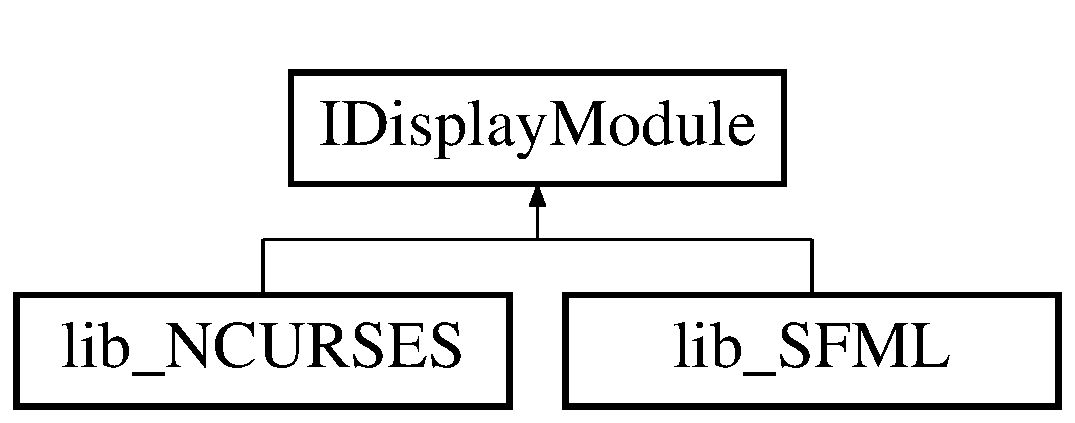
\includegraphics[height=2.000000cm]{class_i_display_module}
\end{center}
\end{figure}
\subsection*{Public Member Functions}
\begin{DoxyCompactItemize}
\item 
\mbox{\label{class_i_display_module_a995de9dca9660bfdcaa5307f473e672c}} 
virtual void {\bfseries Create\+Window} ()=0
\item 
\mbox{\label{class_i_display_module_a95c05ec4c3c59321c67f7b3a9d438dcc}} 
virtual int {\bfseries Refresh} (int value)=0
\item 
\mbox{\label{class_i_display_module_a9952028053323ae0c4841991bc78cf29}} 
virtual int {\bfseries draw\+\_\+map} (map$<$ string, int $>$ mapper)=0
\item 
\mbox{\label{class_i_display_module_ab5d4dce7e501cecaedd6432dd3d82910}} 
virtual void {\bfseries draw\+\_\+content} (\textbf{ t\+\_\+draw\+\_\+data} $\ast$)=0
\item 
\mbox{\label{class_i_display_module_abed5ec651d2c12334c33dff062184dee}} 
virtual int {\bfseries moove} ()=0
\item 
\mbox{\label{class_i_display_module_a1131abc4609bd965e5d598da4d572532}} 
virtual void {\bfseries setnewpos} (\textbf{ t\+\_\+draw\+\_\+data} $\ast$)=0
\item 
\mbox{\label{class_i_display_module_a9e7a55e19b6b5da5f403ec206871f7d8}} 
virtual float {\bfseries get\+Width} (void)=0
\item 
\mbox{\label{class_i_display_module_ad4c80704672cf4217fa144fb0d905e16}} 
virtual float {\bfseries get\+Height} (void)=0
\item 
\mbox{\label{class_i_display_module_acfe514ad0bc31d00a9e092fe8d47324b}} 
virtual void {\bfseries create\+\_\+menu} ()=0
\item 
\mbox{\label{class_i_display_module_a7b730b2a68c4f8d21b79a7788b169468}} 
virtual int {\bfseries select\+\_\+game} (int)=0
\item 
\mbox{\label{class_i_display_module_a8ed6fec6d9c16f0444b7cdadad0f1309}} 
virtual void {\bfseries generate\+\_\+ennemy} (\textbf{ t\+\_\+draw\+\_\+data} $\ast$)=0
\item 
\mbox{\label{class_i_display_module_ad4ec94dc50603d37333d704a3488cfbb}} 
virtual void {\bfseries generate\+\_\+laser} (\textbf{ t\+\_\+draw\+\_\+data} $\ast$)=0
\item 
\mbox{\label{class_i_display_module_afa2cba3aa5b542fe047525ff970f0847}} 
virtual void {\bfseries generate\+\_\+pow} (\textbf{ t\+\_\+draw\+\_\+data} $\ast$content)=0
\end{DoxyCompactItemize}
\subsection*{Protected Attributes}
\begin{DoxyCompactItemize}
\item 
\mbox{\label{class_i_display_module_a61ab3e9d06d2f2ea4165e66cab65acd8}} 
\textbf{ player} $\ast$ {\bfseries p}
\item 
\mbox{\label{class_i_display_module_a87602603ec66bb5e11bfded7d66f8189}} 
vector$<$ \textbf{ player} $\ast$ $>$ $\ast$ {\bfseries secondary}
\item 
\mbox{\label{class_i_display_module_a45dc09e165d015ef164ba1a71823b4f1}} 
vector$<$ \textbf{ player} $\ast$ $>$ $\ast$ {\bfseries tertiary}
\item 
\mbox{\label{class_i_display_module_acbb3def987e9bcb4a1db2c0830bae976}} 
vector$<$ pair$<$ int, int $>$ $>$ $\ast$ {\bfseries quaternary}
\end{DoxyCompactItemize}


The documentation for this class was generated from the following file\+:\begin{DoxyCompactItemize}
\item 
include/I\+Display\+Module.\+hpp\end{DoxyCompactItemize}

\section{I\+Load\+Game Class Reference}
\label{class_i_load_game}\index{I\+Load\+Game@{I\+Load\+Game}}
Inheritance diagram for I\+Load\+Game\+:\begin{figure}[H]
\begin{center}
\leavevmode
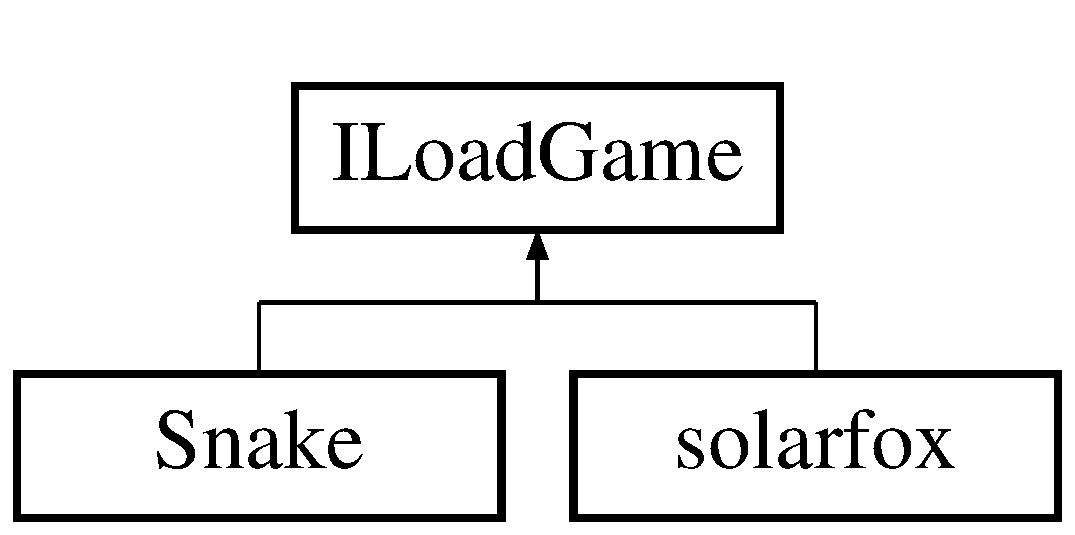
\includegraphics[height=2.000000cm]{class_i_load_game}
\end{center}
\end{figure}
\subsection*{Public Member Functions}
\begin{DoxyCompactItemize}
\item 
\mbox{\label{class_i_load_game_a7b0ecdf2435afe4393ee2eda80e041b1}} 
virtual map$<$ string, int $>$ {\bfseries map\+Creator} (float, float)=0
\item 
\mbox{\label{class_i_load_game_a90e4280011e2355cf9bc4b056aac5afd}} 
virtual \textbf{ t\+\_\+draw\+\_\+data} $\ast$ {\bfseries generate\+Content} (void)=0
\item 
\mbox{\label{class_i_load_game_aa3a2a3d662df1b77f9bbba71ec4f6473}} 
virtual void {\bfseries move\+\_\+player} (\textbf{ player} $\ast$, int)=0
\item 
\mbox{\label{class_i_load_game_a6ecb2016de0b1184ab8d289994fca9a1}} 
virtual void {\bfseries action} (\textbf{ player} $\ast$, int)=0
\item 
\mbox{\label{class_i_load_game_ae394034ebc67308547b8eded51dd4224}} 
virtual int {\bfseries check\+\_\+pos} (void)=0
\item 
\mbox{\label{class_i_load_game_a1b1c75a94ed268bd46034ea92696e40b}} 
virtual \textbf{ player} $\ast$ {\bfseries get\+Player} (void) const =0
\item 
\mbox{\label{class_i_load_game_add53f0396106e6a3ea39f11b0f165aa0}} 
virtual vector$<$ \textbf{ player} $\ast$ $>$ $\ast$ {\bfseries get\+Secondary} (void) const =0
\item 
\mbox{\label{class_i_load_game_a7bf04b5bbf70db852696df005ec70882}} 
virtual vector$<$ \textbf{ player} $\ast$ $>$ $\ast$ {\bfseries get\+Tertiary} (void) const =0
\item 
\mbox{\label{class_i_load_game_a28a272dbda6b0dbc21c704af561016f2}} 
virtual vector$<$ pair$<$ int, int $>$ $>$ $\ast$ {\bfseries get\+Quaternary} (void) const =0
\item 
\mbox{\label{class_i_load_game_a6cd96e642d48d7916c3c378438070ac4}} 
virtual vector$<$ \textbf{ player} $\ast$ $>$ $\ast$ {\bfseries get\+Fifth} (void) const =0
\item 
\mbox{\label{class_i_load_game_afc39bc729987f1d801617bc4486e77c3}} 
virtual bool {\bfseries get\+Game\+Over} () const =0
\item 
\mbox{\label{class_i_load_game_ad4147480ea7dcebdc71869a83d77a921}} 
virtual void {\bfseries game} ()=0
\end{DoxyCompactItemize}
\subsection*{Protected Attributes}
\begin{DoxyCompactItemize}
\item 
\mbox{\label{class_i_load_game_a6a804cef122ad96b599d3affc6eeb6df}} 
\textbf{ player} $\ast$ {\bfseries p}
\item 
\mbox{\label{class_i_load_game_a10a78df6b8a4a4d4f3147885a54f390a}} 
vector$<$ \textbf{ player} $\ast$ $>$ $\ast$ {\bfseries secondary}
\item 
\mbox{\label{class_i_load_game_a27cf0eaecf3beca07ccc334c8717dc99}} 
vector$<$ \textbf{ player} $\ast$ $>$ $\ast$ {\bfseries tertiary}
\item 
\mbox{\label{class_i_load_game_a0a0453bd024995e7a06409eb72220306}} 
vector$<$ pair$<$ int, int $>$ $>$ $\ast$ {\bfseries quaternary}
\item 
\mbox{\label{class_i_load_game_af55d5295be24b48d10124a7188b96953}} 
vector$<$ \textbf{ player} $\ast$ $>$ $\ast$ {\bfseries fifth}
\item 
\mbox{\label{class_i_load_game_a04c1994e5e13c43f691bbd697e08b1aa}} 
map$<$ string, int $>$ {\bfseries Map}
\item 
\mbox{\label{class_i_load_game_ad102429eafd4f3ac825ecc86bf63f73b}} 
bool {\bfseries game\+Over}
\item 
\mbox{\label{class_i_load_game_a75531d37b6221098135305a95702bcf9}} 
float {\bfseries width}
\item 
\mbox{\label{class_i_load_game_a834ad5275c2bb2203aeae90ef8955592}} 
float {\bfseries height}
\end{DoxyCompactItemize}


The documentation for this class was generated from the following file\+:\begin{DoxyCompactItemize}
\item 
include/I\+Load\+Games.\+hpp\end{DoxyCompactItemize}

\section{lib\+\_\+\+N\+C\+U\+R\+S\+ES Class Reference}
\label{classlib___n_c_u_r_s_e_s}\index{lib\+\_\+\+N\+C\+U\+R\+S\+ES@{lib\+\_\+\+N\+C\+U\+R\+S\+ES}}
Inheritance diagram for lib\+\_\+\+N\+C\+U\+R\+S\+ES\+:\begin{figure}[H]
\begin{center}
\leavevmode
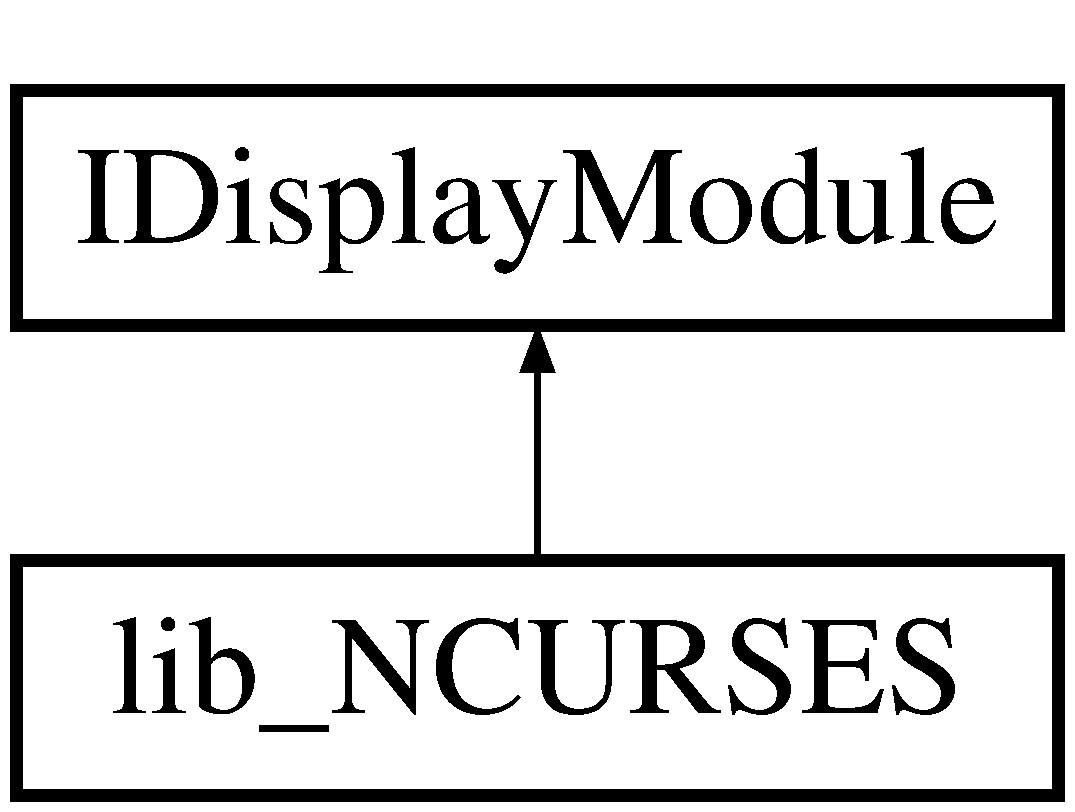
\includegraphics[height=2.000000cm]{classlib___n_c_u_r_s_e_s}
\end{center}
\end{figure}
\subsection*{Public Member Functions}
\begin{DoxyCompactItemize}
\item 
\mbox{\label{classlib___n_c_u_r_s_e_s_a4e2b18378fc2f8e137450e1ce204ab03}} 
void {\bfseries Create\+Window} ()
\item 
\mbox{\label{classlib___n_c_u_r_s_e_s_a74e4f4b1e3b127fa9a0acc40ab01796e}} 
int {\bfseries Refresh} (int value)
\item 
\mbox{\label{classlib___n_c_u_r_s_e_s_a3ebfea69ca0b0cc90be5bef4f3bb0827}} 
int {\bfseries draw\+\_\+map} (map$<$ string, int $>$ mapper)
\item 
\mbox{\label{classlib___n_c_u_r_s_e_s_aa1be8bdce0b43949cddfa0596c3e8651}} 
void {\bfseries draw\+\_\+content} (\textbf{ t\+\_\+draw\+\_\+data} $\ast$)
\item 
\mbox{\label{classlib___n_c_u_r_s_e_s_ae4b417576565df165b47f08f87313e56}} 
int {\bfseries moove} ()
\item 
\mbox{\label{classlib___n_c_u_r_s_e_s_a3443375019352383bb3162a26c990bc3}} 
void {\bfseries setnewpos} (\textbf{ t\+\_\+draw\+\_\+data} $\ast$)
\item 
\mbox{\label{classlib___n_c_u_r_s_e_s_a340d17967c5d4a9a53e60f9903d19537}} 
float {\bfseries get\+Width} (void)
\item 
\mbox{\label{classlib___n_c_u_r_s_e_s_a35d9e822c9d082583a1919afcc047ca1}} 
float {\bfseries get\+Height} (void)
\item 
\mbox{\label{classlib___n_c_u_r_s_e_s_a7e352deb80bbf27cd05355f407416361}} 
void {\bfseries create\+\_\+menu} ()
\item 
\mbox{\label{classlib___n_c_u_r_s_e_s_a2020dbc7ac13eaaf09f63025b783094e}} 
int {\bfseries select\+\_\+game} (int)
\item 
\mbox{\label{classlib___n_c_u_r_s_e_s_a357d104d6d2aa8e3e42479eb5dc19a79}} 
void {\bfseries generate\+\_\+ennemy} (\textbf{ t\+\_\+draw\+\_\+data} $\ast$)
\item 
\mbox{\label{classlib___n_c_u_r_s_e_s_a6c5b3ee239481d6d9cb022e152b77052}} 
void {\bfseries generate\+\_\+laser} (\textbf{ t\+\_\+draw\+\_\+data} $\ast$)
\item 
\mbox{\label{classlib___n_c_u_r_s_e_s_ab1e17e1c0e0c288261f0558cc7d1458f}} 
void {\bfseries generate\+\_\+pow} (\textbf{ t\+\_\+draw\+\_\+data} $\ast$content)
\end{DoxyCompactItemize}
\subsection*{Protected Attributes}
\begin{DoxyCompactItemize}
\item 
\mbox{\label{classlib___n_c_u_r_s_e_s_acba01d3cd85fa065bc3c11910cdda309}} 
int {\bfseries width}
\item 
\mbox{\label{classlib___n_c_u_r_s_e_s_aa08f865dfb9cc6835ff16acb0a34a65b}} 
int {\bfseries height}
\item 
\mbox{\label{classlib___n_c_u_r_s_e_s_ab428ae6d821c70906f24dc8748795122}} 
W\+I\+N\+D\+OW $\ast$ {\bfseries boite}
\item 
\mbox{\label{classlib___n_c_u_r_s_e_s_ac64a42181550a327cc96ab76ca821491}} 
W\+I\+N\+D\+OW $\ast$ {\bfseries title}
\item 
\mbox{\label{classlib___n_c_u_r_s_e_s_a6df8ab15e3f9490e787772e89b597e17}} 
W\+I\+N\+D\+OW $\ast$ {\bfseries solarfox}
\item 
\mbox{\label{classlib___n_c_u_r_s_e_s_a2192fd721f64e153103466a594587e6a}} 
W\+I\+N\+D\+OW $\ast$ {\bfseries snake}
\item 
\mbox{\label{classlib___n_c_u_r_s_e_s_a5a1139cdb112a6870a32310e12d75360}} 
W\+I\+N\+D\+OW $\ast$ {\bfseries map\+\_\+game}
\item 
\mbox{\label{classlib___n_c_u_r_s_e_s_a7d7217630e1047ed32ab9537632c03d5}} 
W\+I\+N\+D\+OW $\ast$ {\bfseries player}
\item 
\mbox{\label{classlib___n_c_u_r_s_e_s_a8c2210a4da28247f3bf0c3b331524059}} 
int {\bfseries key}
\item 
\mbox{\label{classlib___n_c_u_r_s_e_s_afc8535cdf6ef0699e0d71be39bb1c890}} 
int {\bfseries player\+\_\+posX}
\item 
\mbox{\label{classlib___n_c_u_r_s_e_s_a99c8b6694269388d8bc60c04ef1900de}} 
int {\bfseries player\+\_\+posY}
\item 
\mbox{\label{classlib___n_c_u_r_s_e_s_aa13e65d035b43e6a574c96aa268efe8c}} 
int {\bfseries toto}
\end{DoxyCompactItemize}


The documentation for this class was generated from the following files\+:\begin{DoxyCompactItemize}
\item 
lib/ncurses/include/libncurses.\+hpp\item 
lib/ncurses/src/libncurses.\+cpp\end{DoxyCompactItemize}

\section{lib\+\_\+\+S\+F\+ML Class Reference}
\label{classlib___s_f_m_l}\index{lib\+\_\+\+S\+F\+ML@{lib\+\_\+\+S\+F\+ML}}
Inheritance diagram for lib\+\_\+\+S\+F\+ML\+:\begin{figure}[H]
\begin{center}
\leavevmode
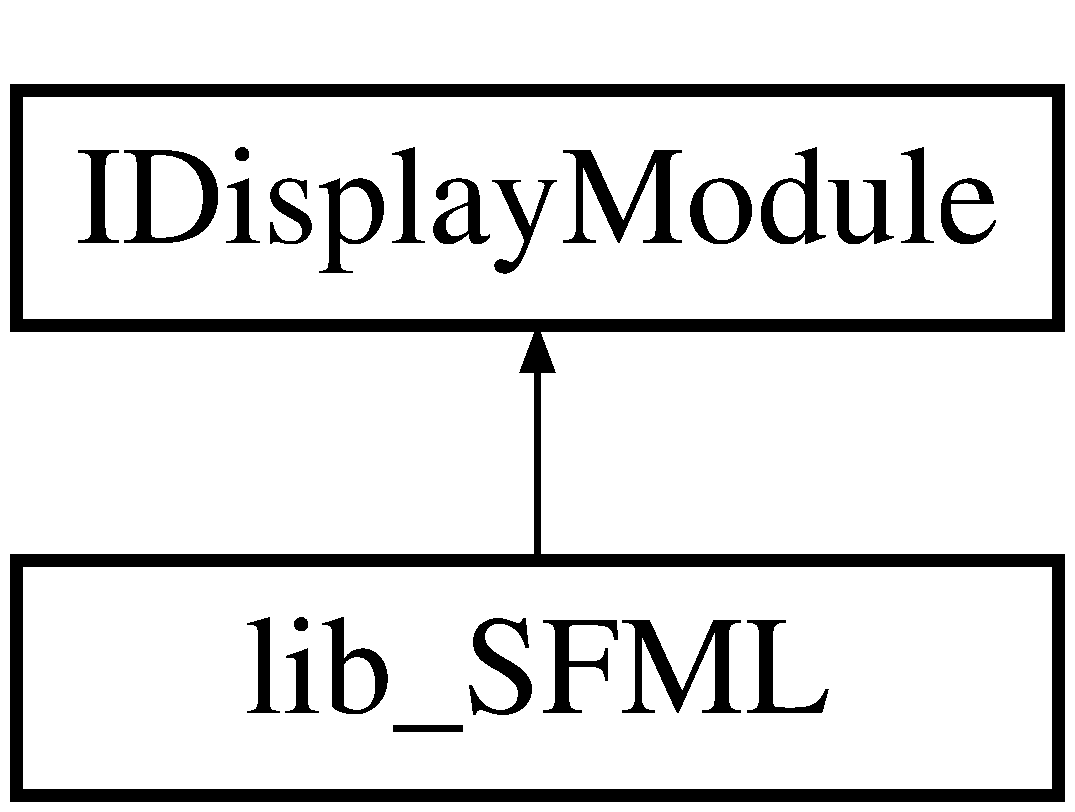
\includegraphics[height=2.000000cm]{classlib___s_f_m_l}
\end{center}
\end{figure}
\subsection*{Classes}
\begin{DoxyCompactItemize}
\item 
struct \textbf{ s\+\_\+textu}
\end{DoxyCompactItemize}
\subsection*{Public Member Functions}
\begin{DoxyCompactItemize}
\item 
\mbox{\label{classlib___s_f_m_l_aa242f45b507422d38b6c035a5af6a70e}} 
int {\bfseries moove} ()
\item 
\mbox{\label{classlib___s_f_m_l_a6a74341595e2c95fac432826cba68638}} 
void {\bfseries Create\+Window} ()
\item 
\mbox{\label{classlib___s_f_m_l_a41fa6d27f86f434e868036633ba7014c}} 
int {\bfseries Refresh} (int value)
\item 
\mbox{\label{classlib___s_f_m_l_a535179537320718a343bc626bd5077ac}} 
int {\bfseries draw\+\_\+map} (map$<$ string, int $>$)
\item 
\mbox{\label{classlib___s_f_m_l_a07ede9b1aacd2684a925ff0fe964d71e}} 
void {\bfseries draw\+\_\+content} (\textbf{ t\+\_\+draw\+\_\+data} $\ast$)
\item 
\mbox{\label{classlib___s_f_m_l_ad4a960c72e8fb1a180adc562152a1b51}} 
void {\bfseries aff\+\_\+map} ()
\item 
\mbox{\label{classlib___s_f_m_l_a978018ecc1bfd5cf9a8cebe1c89a9914}} 
void {\bfseries setnewpos} (\textbf{ t\+\_\+draw\+\_\+data} $\ast$)
\item 
\mbox{\label{classlib___s_f_m_l_a38ab76530c8700126a8ad66683c137fc}} 
void {\bfseries change\+\_\+player} (int, int, int, int)
\item 
\mbox{\label{classlib___s_f_m_l_a1f1da52733f7a9fb5d9a825c6ff7fe0a}} 
float {\bfseries get\+Width} (void)
\item 
\mbox{\label{classlib___s_f_m_l_a28b33b20c2b137175c34c18c150ffd4f}} 
float {\bfseries get\+Height} (void)
\item 
\mbox{\label{classlib___s_f_m_l_aa9441eadb6bee52c7b77a01ab9b8cca4}} 
vector$<$ \textbf{ stocking} $>$ {\bfseries spritor} (string img, int $\ast$value)
\item 
\mbox{\label{classlib___s_f_m_l_ab68be20253e90707e120349c61f1fda7}} 
void {\bfseries create\+\_\+menu} ()
\item 
\mbox{\label{classlib___s_f_m_l_a941f2c7b6232d89c3716a4e3af1d02c1}} 
sf\+::\+Text {\bfseries set\+Text} (float pos\+\_\+x, float pos\+\_\+y, float size, string Text)
\item 
\mbox{\label{classlib___s_f_m_l_a3d1fbad3f243b1ae9c520836cb9f7607}} 
int {\bfseries select\+\_\+game} (int value)
\item 
\mbox{\label{classlib___s_f_m_l_a8fc700af68afc8f1c41a7d118126ad4a}} 
void {\bfseries aff\+\_\+menu} ()
\item 
\mbox{\label{classlib___s_f_m_l_abc745ea0beb2c35824f4c346f402e0c0}} 
void {\bfseries generate\+\_\+ennemy} (\textbf{ t\+\_\+draw\+\_\+data} $\ast$)
\item 
\mbox{\label{classlib___s_f_m_l_a52b0e4a47cb5dcbc9b846653636b5bde}} 
void {\bfseries generate\+\_\+laser} (\textbf{ t\+\_\+draw\+\_\+data} $\ast$)
\item 
\mbox{\label{classlib___s_f_m_l_a40ad910246ade260212ac705e275fb0b}} 
void {\bfseries controle\+\_\+pow} (\textbf{ t\+\_\+draw\+\_\+data} $\ast$content, int number)
\item 
\mbox{\label{classlib___s_f_m_l_a80d61a769246ccbe4f5ce4b94e8e4c15}} 
void {\bfseries controle} (\textbf{ t\+\_\+draw\+\_\+data} $\ast$content, int number)
\item 
\mbox{\label{classlib___s_f_m_l_a068f012264062a1d44c9855831138c0c}} 
int {\bfseries indicate\+\_\+direction} (int direction\+\_\+receive)
\item 
\mbox{\label{classlib___s_f_m_l_a3f50450c16f23ec265e25257e1076a14}} 
void {\bfseries generate\+\_\+pow} (\textbf{ t\+\_\+draw\+\_\+data} $\ast$content)
\end{DoxyCompactItemize}
\subsection*{Protected Types}
\begin{DoxyCompactItemize}
\item 
\mbox{\label{classlib___s_f_m_l_a01308ab6d94978b9f3266126ce7f0e9c}} 
typedef struct \textbf{ lib\+\_\+\+S\+F\+M\+L\+::s\+\_\+textu} {\bfseries t\+\_\+textu}
\end{DoxyCompactItemize}
\subsection*{Protected Attributes}
\begin{DoxyCompactItemize}
\item 
\mbox{\label{classlib___s_f_m_l_acafec6ffbb2e611589c86984b5eed1bd}} 
sf\+::\+Rectangle\+Shape {\bfseries rectangle}
\item 
\mbox{\label{classlib___s_f_m_l_aad136da1b888c789b561be0c643e9165}} 
sf\+::\+Rectangle\+Shape {\bfseries line\+\_\+haut}
\item 
\mbox{\label{classlib___s_f_m_l_a65f596bcc1c07ac5b271e21e09609845}} 
sf\+::\+Rectangle\+Shape {\bfseries line\+\_\+droite}
\item 
\mbox{\label{classlib___s_f_m_l_a4ea65c78097fa73046d2b3a322cc5045}} 
sf\+::\+Rectangle\+Shape {\bfseries line\+\_\+gauche}
\item 
\mbox{\label{classlib___s_f_m_l_a799f84863c9ef05c6f620530088bbfdc}} 
sf\+::\+Rectangle\+Shape {\bfseries line\+\_\+bas}
\item 
\mbox{\label{classlib___s_f_m_l_a5d6b2cd8879e0dda20dea1341d7d2550}} 
sf\+::\+Texture {\bfseries texture\+\_\+player}
\item 
\mbox{\label{classlib___s_f_m_l_a6bb9e3f74b68de7512388ec33356829c}} 
sf\+::\+Sprite {\bfseries sprite\+\_\+player}
\item 
\mbox{\label{classlib___s_f_m_l_a961c979490e59236ef1fd7ae7064ce10}} 
sf\+::\+Render\+Window {\bfseries window}
\item 
\mbox{\label{classlib___s_f_m_l_ad58b75107373a0be34ba08880ccfb65f}} 
vector$<$ float $>$ {\bfseries save\+\_\+player}
\item 
\mbox{\label{classlib___s_f_m_l_abd39e8150e6ab622abc624aadfab3111}} 
sf\+::\+Texture {\bfseries textu\+\_\+back}
\item 
\mbox{\label{classlib___s_f_m_l_a5ba69bf2a680ca2ac61098cd8a8372e6}} 
sf\+::\+Sprite {\bfseries sprite\+\_\+back}
\item 
\mbox{\label{classlib___s_f_m_l_a3992dadf817d4f71f0edf8a16f9ff8a9}} 
sf\+::\+Font {\bfseries font\+\_\+menu}
\item 
\mbox{\label{classlib___s_f_m_l_affa7ca82c3ec4a531d8059011febbb86}} 
sf\+::\+Text {\bfseries text\+\_\+menu}
\item 
\mbox{\label{classlib___s_f_m_l_afab51dda4a7193ec1ba6d8769d28a65d}} 
sf\+::\+Text {\bfseries text\+\_\+snake}
\item 
\mbox{\label{classlib___s_f_m_l_af66b3764239afeb27c6c0a9c6eacb989}} 
sf\+::\+Text {\bfseries text\+\_\+solar}
\item 
\mbox{\label{classlib___s_f_m_l_a5f41388899a22cb76000059e479857b1}} 
vector$<$ \textbf{ stocking} $>$ {\bfseries maine}
\item 
\mbox{\label{classlib___s_f_m_l_aa54860ebe7208b90d54baa7cd90c4f8c}} 
vector$<$ \textbf{ stocking} $>$ {\bfseries corp}
\item 
\mbox{\label{classlib___s_f_m_l_aadde055784a26ffa3568215ca9d9695d}} 
vector$<$ \textbf{ stocking} $>$ {\bfseries last}
\item 
\mbox{\label{classlib___s_f_m_l_a4ac1aa1ea9f1d9f26e4f670ff4d7cee5}} 
vector$<$ \textbf{ stocking} $>$ {\bfseries data}
\item 
\mbox{\label{classlib___s_f_m_l_a1c15cdc966707bc825316d5b167d467c}} 
vector$<$ \textbf{ stocking} $>$ {\bfseries pow}
\item 
\mbox{\label{classlib___s_f_m_l_aa20eee9d5c605bc86a651d7f5d4b9535}} 
\textbf{ stocking} {\bfseries tmp} [20]
\item 
\mbox{\label{classlib___s_f_m_l_a5b39bb40b18845cdbe77a5a74a7ec7cc}} 
vector$<$ sf\+::\+Sprite $>$ {\bfseries ennemy}
\item 
\mbox{\label{classlib___s_f_m_l_a9c6277114ed3abeb3c42ded632328bfd}} 
vector$<$ sf\+::\+Sprite $>$ {\bfseries laser}
\item 
\mbox{\label{classlib___s_f_m_l_aed512c3da6f669cd4be12062351d4ec9}} 
vector$<$ sf\+::\+Sprite $>$ {\bfseries power}
\item 
\mbox{\label{classlib___s_f_m_l_af4b6b3def3a89126bb1a91b270041e85}} 
sf\+::\+Event {\bfseries event}
\item 
\mbox{\label{classlib___s_f_m_l_ac2c536cf9117135be3587f28106af61c}} 
int {\bfseries way}
\item 
\mbox{\label{classlib___s_f_m_l_ac214779b48b8e9a98d7adf439213720d}} 
int {\bfseries width}
\item 
\mbox{\label{classlib___s_f_m_l_a6954a15233f24a9315c3529ad35bec13}} 
int {\bfseries height}
\item 
\mbox{\label{classlib___s_f_m_l_ac5eb266da535c466674280b0492df6f6}} 
vector$<$ sf\+::\+Sprite $>$ {\bfseries sprite\+\_\+game}
\item 
\mbox{\label{classlib___s_f_m_l_a376ae168692c1555132f3c1f05319c5a}} 
vector$<$ sf\+::\+Texture $>$ {\bfseries textu\+\_\+game}
\end{DoxyCompactItemize}


The documentation for this class was generated from the following files\+:\begin{DoxyCompactItemize}
\item 
lib/include/libsfml.\+hpp\item 
lib/src/display.\+cpp\item 
lib/src/drawer.\+cpp\item 
lib/src/generateur.\+cpp\item 
lib/src/getter.\+cpp\item 
lib/src/libsfml.\+cpp\item 
lib/src/menu.\+cpp\item 
lib/src/window.\+cpp\end{DoxyCompactItemize}

\section{player Class Reference}
\label{classplayer}\index{player@{player}}
\subsection*{Public Member Functions}
\begin{DoxyCompactItemize}
\item 
\mbox{\label{classplayer_a1bb8a7a0826319d6478fdc8d0646cb44}} 
{\bfseries player} (float, float, int)
\item 
\mbox{\label{classplayer_a0d21f3a93f19e8db64c292041a9df741}} 
float {\bfseries turn\+Drawable} (void)
\item 
\mbox{\label{classplayer_a94780f0cab9b7bc64b96c41a5eda37f5}} 
float {\bfseries get\+PosX} (void) const
\item 
\mbox{\label{classplayer_aa05fc23c830ab8aa9ac0d501cc373437}} 
float {\bfseries get\+PosY} (void) const
\item 
\mbox{\label{classplayer_a7b4e77c30b428491542d4db67f8a730a}} 
float $\ast$ {\bfseries get\+Pos} (void) const
\item 
\mbox{\label{classplayer_a979ab94d5734e9f1403c5ca10b749c86}} 
int {\bfseries get\+Way} (void) const
\item 
\mbox{\label{classplayer_a8022861762da457945c438567a7a292f}} 
void {\bfseries set\+PosX} (float)
\item 
\mbox{\label{classplayer_a5e0d3eec1d24faac4f091f21a6ec767b}} 
void {\bfseries set\+PosY} (float)
\item 
\mbox{\label{classplayer_a42b4e39d4c428aa504e576cb3af7d759}} 
void {\bfseries set\+Way} (float)
\item 
\mbox{\label{classplayer_a85c3a6aeae5fc828c795d4e07d6f09ce}} 
void {\bfseries forward} ()
\item 
\mbox{\label{classplayer_a80aa9976bf0ea61ca1ed0e140a5179d1}} 
int {\bfseries is\+On\+Edge} (float, float)
\end{DoxyCompactItemize}
\subsection*{Protected Attributes}
\begin{DoxyCompactItemize}
\item 
\mbox{\label{classplayer_aa90eebef283ae699474d11673aa55f31}} 
float {\bfseries x}
\item 
\mbox{\label{classplayer_aad2d959f61d8eaf5f75bd38d9fc6784d}} 
float {\bfseries y}
\item 
\mbox{\label{classplayer_afbef4efdba300b6b8aa6d07b31b124d1}} 
int {\bfseries way}
\end{DoxyCompactItemize}


The documentation for this class was generated from the following files\+:\begin{DoxyCompactItemize}
\item 
include/player.\+hpp\item 
src/player/checkpos.\+cpp\item 
src/player/constructor.\+cpp\item 
src/player/getter.\+cpp\item 
src/player/move.\+cpp\item 
src/player/setter.\+cpp\end{DoxyCompactItemize}

\section{s\+\_\+core Struct Reference}
\label{structs__core}\index{s\+\_\+core@{s\+\_\+core}}
\subsection*{Public Attributes}
\begin{DoxyCompactItemize}
\item 
\mbox{\label{structs__core_ad77d662a6349440d2c414b0874b16562}} 
void $\ast$ {\bfseries handler}
\item 
\mbox{\label{structs__core_aa70da68357d19de866adadab0fdc5c8c}} 
create\+\_\+t $\ast$ {\bfseries create}
\item 
\mbox{\label{structs__core_a8aaef7788fcdd4e3684714486c7f5dc0}} 
destroy\+\_\+t $\ast$ {\bfseries destroy}
\item 
\mbox{\label{structs__core_af333475be6031916e6d2cae13bd52f8d}} 
create\+\_\+us $\ast$ {\bfseries create\+\_\+games}
\item 
\mbox{\label{structs__core_a4ad162483bde6a04c8743987f0bea287}} 
destroy\+\_\+us $\ast$ {\bfseries destroy\+\_\+games}
\item 
\mbox{\label{structs__core_a6b62d1e9e55a47a22159854074c06c8f}} 
const char $\ast$ {\bfseries dlsym\+\_\+error}
\item 
\mbox{\label{structs__core_a8573db6f1eba9454687fa0b8af897313}} 
\textbf{ I\+Display\+Module} $\ast$ {\bfseries display}
\item 
\mbox{\label{structs__core_a857af41c606dbd822b76b64a18714768}} 
\textbf{ I\+Load\+Game} $\ast$ {\bfseries gaming}
\end{DoxyCompactItemize}


The documentation for this struct was generated from the following file\+:\begin{DoxyCompactItemize}
\item 
include/Core.\+hpp\end{DoxyCompactItemize}

\section{s\+\_\+draw\+\_\+data Struct Reference}
\label{structs__draw__data}\index{s\+\_\+draw\+\_\+data@{s\+\_\+draw\+\_\+data}}
\subsection*{Public Attributes}
\begin{DoxyCompactItemize}
\item 
\mbox{\label{structs__draw__data_a3800961e5f73ac08f8cc85bc9ac63877}} 
\textbf{ player} $\ast$ {\bfseries p}
\item 
\mbox{\label{structs__draw__data_acf538c8d6ad30424795acb326ca52d8e}} 
vector$<$ \textbf{ player} $\ast$ $>$ $\ast$ {\bfseries secondary}
\item 
\mbox{\label{structs__draw__data_a3db1990ea223075020306acbd83d0e58}} 
vector$<$ \textbf{ player} $\ast$ $>$ $\ast$ {\bfseries tertiary}
\item 
\mbox{\label{structs__draw__data_aa73d7ce059f266a170139e95302b1356}} 
vector$<$ pair$<$ int, int $>$ $>$ $\ast$ {\bfseries quaternary}
\item 
\mbox{\label{structs__draw__data_a499216d35b2c5b5329b7dfa9a66d69ec}} 
map$<$ string, int $>$ {\bfseries Map}
\item 
\mbox{\label{structs__draw__data_a2c856a6ad18d8973e7756b05b18a0e75}} 
vector$<$ \textbf{ player} $\ast$ $>$ $\ast$ {\bfseries fifth}
\item 
\mbox{\label{structs__draw__data_a410c5a6660eb4b7c3a03684b6cfd564f}} 
string {\bfseries sprite}
\end{DoxyCompactItemize}


The documentation for this struct was generated from the following file\+:\begin{DoxyCompactItemize}
\item 
include/player.\+hpp\end{DoxyCompactItemize}

\section{s\+\_\+stock Struct Reference}
\label{structs__stock}\index{s\+\_\+stock@{s\+\_\+stock}}
\subsection*{Public Attributes}
\begin{DoxyCompactItemize}
\item 
\mbox{\label{structs__stock_a75f91cfc81272ec7839adfa9317a5fc2}} 
sf\+::\+Sprite {\bfseries sprite\+\_\+game}
\item 
\mbox{\label{structs__stock_a9252a7d071788536be1d5110f6cdc9a0}} 
sf\+::\+Texture {\bfseries textu\+\_\+game}
\end{DoxyCompactItemize}


The documentation for this struct was generated from the following file\+:\begin{DoxyCompactItemize}
\item 
lib/include/libsfml.\+hpp\end{DoxyCompactItemize}

\section{lib\+\_\+\+S\+F\+ML\+:\+:s\+\_\+textu Struct Reference}
\label{structlib___s_f_m_l_1_1s__textu}\index{lib\+\_\+\+S\+F\+M\+L\+::s\+\_\+textu@{lib\+\_\+\+S\+F\+M\+L\+::s\+\_\+textu}}
\subsection*{Public Attributes}
\begin{DoxyCompactItemize}
\item 
\mbox{\label{structlib___s_f_m_l_1_1s__textu_a6e7497bb324d6ee127d3fe8af82b7a2b}} 
int {\bfseries pos\+\_\+img\+\_\+x} = 0
\item 
\mbox{\label{structlib___s_f_m_l_1_1s__textu_a8ed5fd3d7656bae6666b5af4c8dfde02}} 
int {\bfseries pos\+\_\+img\+\_\+y} = 0
\item 
\mbox{\label{structlib___s_f_m_l_1_1s__textu_af152c7de9fa637cfe8147541856eb41b}} 
int {\bfseries longu} = 65
\item 
\mbox{\label{structlib___s_f_m_l_1_1s__textu_a2948a6100bc539a45dd53517096f9c51}} 
int {\bfseries larg} = 65
\end{DoxyCompactItemize}


The documentation for this struct was generated from the following file\+:\begin{DoxyCompactItemize}
\item 
lib/include/libsfml.\+hpp\end{DoxyCompactItemize}

\section{Snake Class Reference}
\label{class_snake}\index{Snake@{Snake}}
Inheritance diagram for Snake\+:\begin{figure}[H]
\begin{center}
\leavevmode
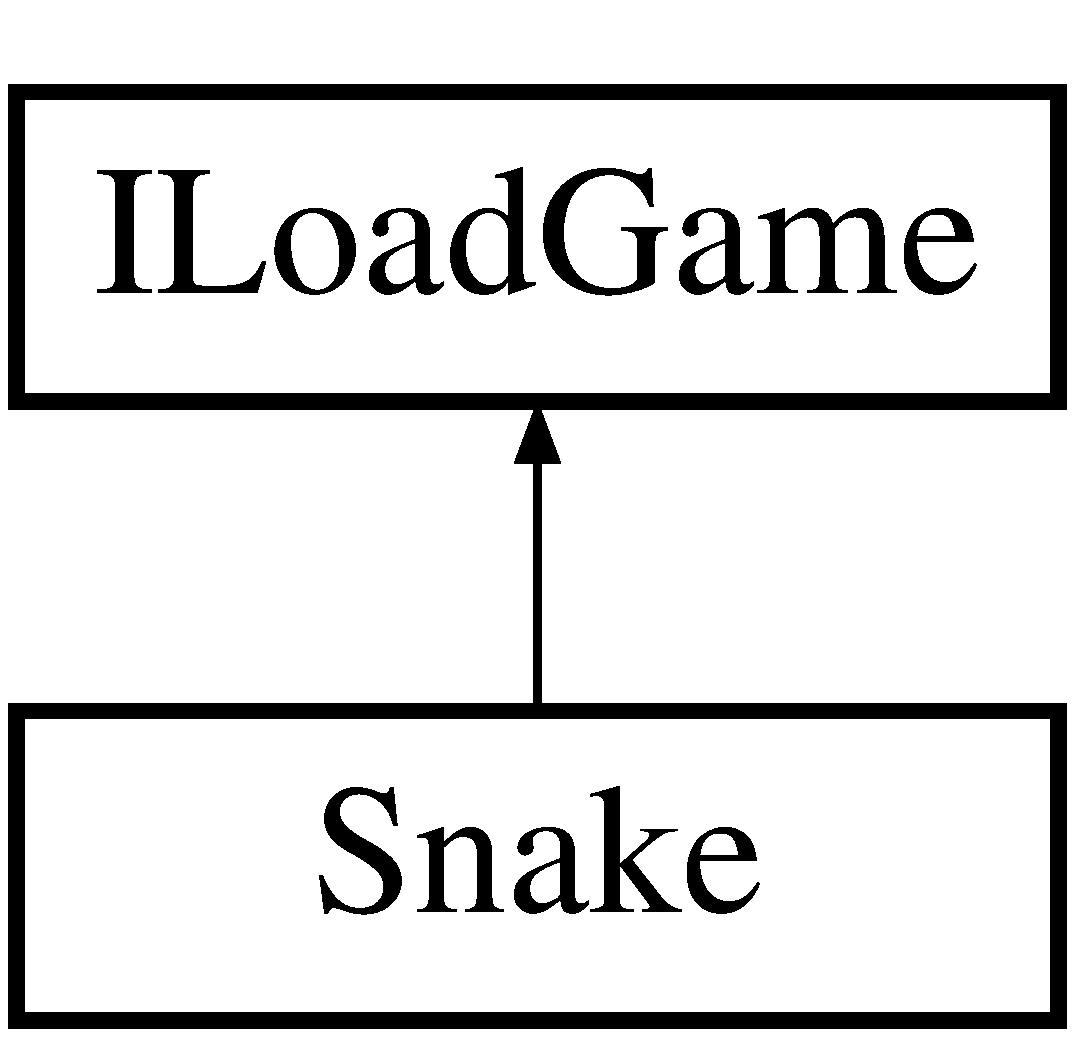
\includegraphics[height=2.000000cm]{class_snake}
\end{center}
\end{figure}
\subsection*{Public Member Functions}
\begin{DoxyCompactItemize}
\item 
\mbox{\label{class_snake_a7b81421e0c7eedf3a7404943d46b616b}} 
virtual map$<$ string, int $>$ {\bfseries map\+Creator} (float, float)
\item 
\mbox{\label{class_snake_a87c85cbe4793ed56e7dc278bce3f3ca0}} 
\textbf{ t\+\_\+draw\+\_\+data} $\ast$ {\bfseries generate\+Content} (void)
\item 
\mbox{\label{class_snake_ac0be7c8da71c7a4502e126e160660a4c}} 
void {\bfseries move\+\_\+player} (\textbf{ player} $\ast$p, int value)
\item 
\mbox{\label{class_snake_a5d5e576f96e28c3e2f3ac60e4d7cf292}} 
\textbf{ player} $\ast$ {\bfseries get\+Player} (void) const
\item 
\mbox{\label{class_snake_a738ac832860df6e3c54fb77cca92e72f}} 
vector$<$ \textbf{ player} $\ast$ $>$ $\ast$ {\bfseries get\+Secondary} (void) const
\item 
\mbox{\label{class_snake_ad8cd4a0377053234f7673f95d6902846}} 
vector$<$ \textbf{ player} $\ast$ $>$ $\ast$ {\bfseries get\+Tertiary} (void) const
\item 
\mbox{\label{class_snake_a2ace77187281c86681fcfca44bf0c7ad}} 
vector$<$ pair$<$ int, int $>$ $>$ $\ast$ {\bfseries get\+Quaternary} (void) const
\item 
\mbox{\label{class_snake_a280b8abdd1156836a1daa00ff6b627e6}} 
vector$<$ \textbf{ player} $\ast$ $>$ $\ast$ {\bfseries get\+Fifth} (void) const
\item 
\mbox{\label{class_snake_ac9d799ff927618a484da4ae14df67ef9}} 
bool {\bfseries get\+Game\+Over} (void) const
\item 
\mbox{\label{class_snake_a31f2fe1bb2175260f2ebb3d2db40a9a7}} 
int {\bfseries check\+\_\+pos} (void)
\item 
\mbox{\label{class_snake_ad10570520301d6d7594d91223996f8d3}} 
void {\bfseries action} (\textbf{ player} $\ast$, int)
\item 
\mbox{\label{class_snake_abe8f046cfd2c717eda99e5c6d7bdcc03}} 
void {\bfseries game} (void)
\item 
\mbox{\label{class_snake_abccbcd3ed8ba522a87c9e429af69e75b}} 
void {\bfseries add\+Fruit} (void)
\item 
\mbox{\label{class_snake_af7ab67615280f5fcfa3153f328717eb4}} 
bool {\bfseries check\+Death} (void)
\item 
\mbox{\label{class_snake_a7bb21a0b691871dffa34adc58d8e6ff0}} 
void {\bfseries pick\+Fruit} (void)
\item 
\mbox{\label{class_snake_ad89cdeb548e6191d760acda1d999c89a}} 
void {\bfseries add\+To\+Tail} (void)
\item 
\mbox{\label{class_snake_a71f06eacde8333272f5042c26b605a11}} 
\textbf{ player} $\ast$ {\bfseries gen\+Tail} (void)
\item 
\mbox{\label{class_snake_a2a47c8ad4c1b45e94afad819d0531752}} 
void {\bfseries gen\+New\+Pos} (vector$<$ \textbf{ player} $\ast$$>$\+::iterator, \textbf{ player} $\ast$)
\end{DoxyCompactItemize}
\subsection*{Additional Inherited Members}


The documentation for this class was generated from the following files\+:\begin{DoxyCompactItemize}
\item 
games/snake/include/snake.\+hpp\item 
games/snake/src/action.\+cpp\item 
games/snake/src/check.\+cpp\item 
games/snake/src/constructor.\+cpp\item 
games/snake/src/fruit.\+cpp\item 
games/snake/src/game.\+cpp\item 
games/snake/src/generate.\+cpp\item 
games/snake/src/getter.\+cpp\item 
games/snake/src/move.\+cpp\end{DoxyCompactItemize}

\section{solarfox Class Reference}
\label{classsolarfox}\index{solarfox@{solarfox}}
Inheritance diagram for solarfox\+:\begin{figure}[H]
\begin{center}
\leavevmode
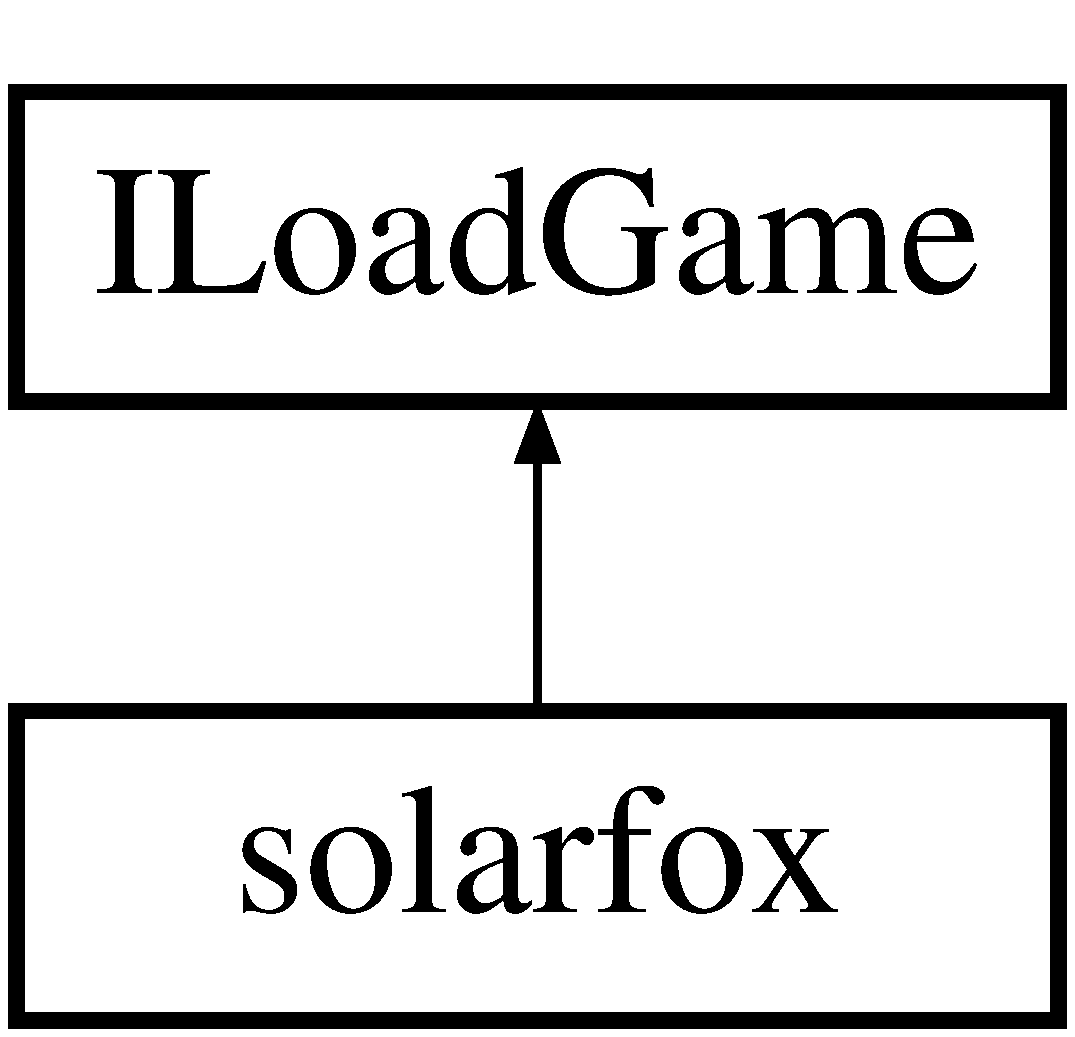
\includegraphics[height=2.000000cm]{classsolarfox}
\end{center}
\end{figure}
\subsection*{Public Member Functions}
\begin{DoxyCompactItemize}
\item 
\mbox{\label{classsolarfox_a395d25edb3da264e01ca7798e80357ab}} 
\textbf{ player} $\ast$ {\bfseries get\+Player} (void) const
\item 
\mbox{\label{classsolarfox_a5b7e761a3135ceab166d44020a8951ab}} 
vector$<$ \textbf{ player} $\ast$ $>$ $\ast$ {\bfseries get\+Secondary} (void) const
\item 
\mbox{\label{classsolarfox_af9fcc28b586985bc8ea47f6036a5801d}} 
vector$<$ \textbf{ player} $\ast$ $>$ $\ast$ {\bfseries get\+Tertiary} (void) const
\item 
\mbox{\label{classsolarfox_a7d2cf72fd374768d04e4dc184da4e406}} 
vector$<$ pair$<$ int, int $>$ $>$ $\ast$ {\bfseries get\+Quaternary} (void) const
\item 
\mbox{\label{classsolarfox_aa6ea976c2b26ac2bf1cccf72af59c769}} 
vector$<$ \textbf{ player} $\ast$ $>$ $\ast$ {\bfseries get\+Fifth} (void) const
\item 
\mbox{\label{classsolarfox_a0104f3fe7bbcaf7510a152fbe3e7e27b}} 
bool {\bfseries get\+Game\+Over} () const
\item 
\mbox{\label{classsolarfox_a6f224bd7f2b60bd8adf1791054d00e93}} 
void {\bfseries game} (void)
\item 
\mbox{\label{classsolarfox_a2612b957b4bc234ec6aa2132699fb50f}} 
void {\bfseries spawner} (void)
\item 
\mbox{\label{classsolarfox_ad324290ede25c99cadb7a62310648ef4}} 
void {\bfseries shoot} (void)
\item 
\mbox{\label{classsolarfox_ab6504ee8365eea828d20e5f5d0e699ec}} 
void {\bfseries launch\+Missile} (void)
\item 
\mbox{\label{classsolarfox_a270a5f4d3f55d8b33f91434920d3a86b}} 
vector$<$ pair$<$ int, int $>$ $>$ $\ast$ {\bfseries gen\+Map} (void)
\item 
\mbox{\label{classsolarfox_ad762204619d4517cf2d5ca788eeaedb5}} 
void {\bfseries move\+\_\+player} (\textbf{ player} $\ast$p, int value)
\item 
\mbox{\label{classsolarfox_a9406fe341b5a325a3ffcd0eb3137407e}} 
int {\bfseries check\+\_\+pos} ()
\item 
\mbox{\label{classsolarfox_ab1f2166fe5607be51d4570a38799e27b}} 
bool {\bfseries check\+Death} (void)
\item 
\mbox{\label{classsolarfox_ad246c43f6d2dee67255072ba2be89e1b}} 
void {\bfseries lasers\+Forward} (void)
\item 
\mbox{\label{classsolarfox_a6b504344dd12a73415d44398ff707e8d}} 
void {\bfseries check\+Collision} (void)
\item 
\mbox{\label{classsolarfox_a8a5ab035998af2e54bbf604c3c78bc3f}} 
void {\bfseries pick\+Powerup} (void)
\item 
\mbox{\label{classsolarfox_a1e4515f7e21deedf0e78162e29c8af48}} 
void {\bfseries clear\+Outside} (void)
\item 
\mbox{\label{classsolarfox_ac4694604f7cbeccd29c5bbcc0b277cde}} 
virtual map$<$ string, int $>$ {\bfseries map\+Creator} (float, float)
\item 
\mbox{\label{classsolarfox_aabce5ca313f8bcdbd41a7903ed9ea738}} 
\textbf{ t\+\_\+draw\+\_\+data} $\ast$ {\bfseries generate\+Content} ()
\item 
\mbox{\label{classsolarfox_a01d97c5df64680bdb82ba2b06e87ae9e}} 
void {\bfseries action} (\textbf{ player} $\ast$, int)
\end{DoxyCompactItemize}
\subsection*{Additional Inherited Members}


The documentation for this class was generated from the following files\+:\begin{DoxyCompactItemize}
\item 
games/solarfox/include/solarfox.\+hpp\item 
games/solarfox/src/constructor.\+cpp\item 
games/solarfox/src/getter.\+cpp\item 
games/solarfox/src/getter2.\+cpp\item 
games/solarfox/src/missile.\+cpp\item 
games/solarfox/src/move.\+cpp\item 
games/solarfox/src/powerup.\+cpp\item 
games/solarfox/src/solarfox.\+cpp\end{DoxyCompactItemize}

%--- End generated contents ---

% Index
\backmatter
\newpage
\phantomsection
\clearemptydoublepage
\addcontentsline{toc}{chapter}{Index}
\printindex

\end{document}
